\documentclass{article}

\usepackage{amsmath}
\usepackage{amssymb}
\usepackage{hyperref}
\usepackage{graphicx}

\graphicspath{ {./} }

\author{Aurora Zuoris \\ \texttt{aurora.zuoris101@alu.ulpgc.es}}

\title{Sparce matrix multiplication}

\begin{document}

\maketitle

\abstract{
Sparce matrices are matrices that have a lot of zero elements,
thus it is possible to save a lot of memory by not storing these zero elements.
This can be beneficial in many applications, such as graph theory, where the adjacency matrix of a graph is sparce.
This paper will explore the different ways of storing sparce matrices and the different ways of multiplying them,
mainly focusing on the CCS and coordinate formats.
}

\section{Introduction}

Sparce matrices are an alternative to dense matrices.
In these matrices, the majority of elements are null, thus it is more efficient to only store the
non null elements rather than all of them. This allows for storing bigger matrices as they consume less memory,
and also may lead to some computational improvements as the algorithms made for these matrices will only look at the existing elements.

\section{Implementations}

There are various ways to implement sparce matrices.
The most obvious one is the coordinate format, in which tuples are stored which indicate the coordinate into the matrix and its value,
such that any coordinate that isn't present is assumed to take on a null value.
Complementing this, the paper will also try to implement an indexed coordinate format, where each matrix keeps indices of the rows and columns
aimed at optimizing iterating these, which may be beneficial for matrix multiplications.
Aditionally there are some other more sophisticated formats, like the CCS and the CRS,
of these two only the CCS will be implemented, as they're basically the same, just a transpose of each other.

All the code used in the paper can be found at \url{https://github.com/Aurora2500/big-data-sparce-matrix}

\subsection{Coordinate format}

Coordinate format consists of storing three-element tuples consisting of the row, column, and value.
To do this, a pair type is implemented that has its own equivalence and hash methods overriden.
Then internally, the matrix class will store a map from pairs to values, allowing for O(1) access operations.

\subsection{Indexed coordinate format}

This format is very similar to the last one, except that it also consists of various indices for the columns and rows,
leading to much more optimized iteration over arbitrary rows and columns.
These are implemented using a map from the corresponding row/column to a set of row/column and value pairs.
This way, when one wants to iterate over a given row, they get an iterator of column/value pairs, and similar
for iterating over a given column.
It is hypothesized that this can be beneficial for matrix multiplication as, the values of the product matrix are the result of the dot product of the rows
and columns of the factor matrices, thus quick iteration over an arbitrary row and or column should be a great improvement.

\subsection{Compressed Column Storage format}

A compressed column (and row) storage format consists of three lists,
a column pointer, a row, and a value list.
For an $n$ by $m$ matrix with $k$ elements,
the column pointer list will consist of $m+1$ elements, the first one being 0
and the last one being $k$, with each element being a monotonically increasing number.
The interpretation of this list is that the $j$th column has $\text{col\_ptr} [j] - \text{col\_ptr} [j-1]$ elements,

corresponding to the elements residing in the other two lists.
The row and value lists will then both have $k$ elements, with each element of the value list being the actual
value residing in the matrix, and the corresponding element in the rows list representing which row that value resides in.
Inserting and removing elements from such a matrix is very impractical, but the lookup is $O(\log(m))$ 
where $m$ is the number of elements in a columnl, as the column can be looked up in constant time,
and then it's a matter of finding the corresponding row, which can be done using binary lookup as long as these are also
ordered monotonically.

Due to the complicated nature of this format and dificulty of online creation, it is often the most feasible to
first create a coordinate matrix to use as an intermediary step for the creation of a matrix in this format.

Due to time constraints, this format couldn't be benchmarked.

\subsection{Testing}

To test these implementations and assert their correctness,
a property based approach is taken, in which each test will
generate a number of randomly generated matrices, and then test that they
follow some property, such as associativity.
This testing approach leads to each test case representing a different mathematical property that the matrices may hold,
which can be good as there's less of a focus on getting a single case correct, as it checks in a wide number of different randomly generated
values, and aditionally these tests won't consist of needing to reimplement the functionality that is being tested,
as is often the case in other approaches, given that testing a property can usually be done with much more simple and expressive code.

\section{Results and conclusions}

\begin{figure}[h!]
	\centering
	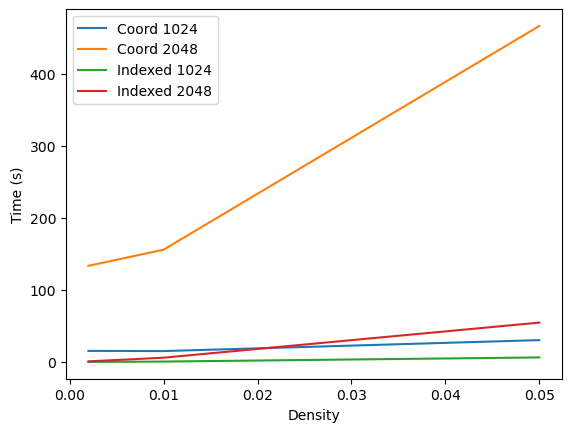
\includegraphics[width=0.8\textwidth]{plot.png}
\end{figure}

As it can be seen, the indexed coordinate format speeds up the multiplication by a factor of up to 100,
which is a very significant improvement.
This is due to it only needing to iterate over the elements that are actually present in the matrix.

More benchmarking needs to be done for a more conclusive result,
but this is a very promising result for just the formats that were implemented.

\section{Future work}

A couple of key missing features from this paper is the
use of a proper benchmarking framework, like JMH.
Aditionally, some formats that were planned like the CCS
couldn't be benchmarked due to time constraints.

In the future, it might be interesting to see even more specialized matrix formats that could be used,
for example for unitary matrices or for symetric matrices,
as these all have their own different optimizations for storage and matrix multiplication, and can still
be used well for various applications when it comes to matters like processing graphs and networks.

\end{document}